\begin{frame}{Level identification in CFT spectra}
\vskip-1.5cm
\begin{columns}[T]
\begin{column}{0.25\textwidth}
\begin{figure}
\scalebox{0.5}{
\begin{tikzpicture}[x=30mm,y=25mm]
\tikzstyle{yaxis} = [-triangle 90]
\tikzstyle{xaxis} = [triangle 90-triangle 90]
\node[inv](A) at (-.5, 0){};
\node[inv](B) at (2.5, 0){};
\draw[thick, xaxis] (A)-- (B);
\node at ($ (A) !.6! (B) +(0, -0.3)$) {\Huge $P$ \Large (in units of $\frac{2\pi}{L}$)};
\node[inv](A) at (0, 0){};
\node[inv](B) at (0, 4){};
\draw[thick, yaxis] (A)--(B);
\node at ($ (A) !.9! (B) +(-0.3, 0)$) {\Huge $E$};

\def\rs{{ 0, 1, 0, .9, 0, 1, 1}}
\def\gs{{0, 0, 0, .5, 1, 1, 0}}
\def\bs{{0, 0, 1, 0, 0, 0, 1}}
\def\decxs{{1,1.95,2.05,0}}
\def\decys{{1, 2,    2, 2}}

\foreach \q in {6, ..., 0}{
\pgfmathparse{\rs[\q]}
\edef\r{\pgfmathresult}

\pgfmathparse{\gs[\q]}
\edef\g{\pgfmathresult}

\pgfmathparse{\bs[\q]}
\edef\b{\pgfmathresult}
\definecolor{mycolor}{rgb}{\r,\g,\b}
\tikzset{spec/.style={circle=2pt,draw=black!100,fill=mycolor!100,inner sep=2pt}}
\node[spec](P\q) at (0, 1/6.2*\q*\q*1/4.0){};
\foreach \k in {0,...,3}{

\pgfmathparse{\decxs[\k]}
\edef\x{\pgfmathresult}
\pgfmathparse{\decys[\k]}
\edef\y{\pgfmathresult}

%\pgfmathtruncatemacro\intx{\x}
%\pgfmathtruncatemacro\inty{\y}

\node[spec](P\q\k) at ($(P\q)+(\x, \y)$){};
%\node[spec](P\q\k) at ($(P\q)+(-\x, \y)$){};
% \newdimen\xx
% \newdimen\yy
% \pgfextractx{\xx}{\pgfpointanchor{P\q\k}{center}}
% \pgfextracty{\yy}{\pgfpointanchor{P\q\k}{center}}
% \pgfmathtruncatemacro\intx{\xx}
% \pgfmathtruncatemacro\inty{\yy}


}
}

\end{tikzpicture}
}
\end{figure}
\end{column}
\begin{column}{0.75\textwidth}
\begin{figure}[hbctp]
\begin{center}
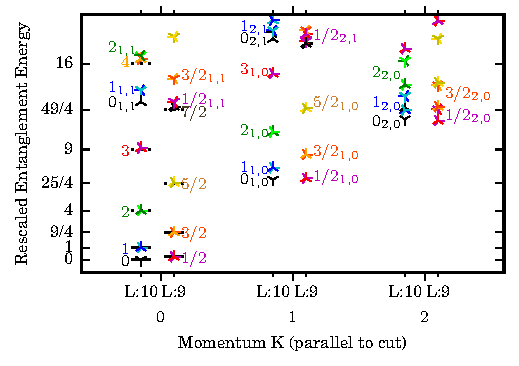
\includegraphics[height=\textheight]{{interpolatedboson/a10/plots/EEIdentify.pdf}}
\end{center}
%\caption{The identification of the states $\ket{e, m}_{n, \bar{n}}$ in the spectrum of the soft-core boson entanglement Hamiltonian. The label $e$ gives the U(1) charge. The labels $n$, $\bar{n}$ label the levels in the right or left-moving sectors of the Kac-Moody algebra. When the level $n$ is larger than 1, the level shows $Z(n)$ approximately degenerate states. The best estimate for the Luttinger parameter $\kappa = 1/6.4$ is given by the inverse of the energy of the $\ket{1, 0}_{1, 0}$ state. The label $m$ is 0 for all states shown - however, the primary states $\ket{e, m=\pm 1}$ can be seen centered around momentum $\pi$, with energies on the order of $1/(4\kappa^2)$.}
%\label{fig:primaries}
\end{figure}
\end{column}
\end{columns}
\end{frame}